% Supplemental Material for the vortex-disruption letter.
%
% Build: make (in this directory). Every number below that comes from a run is
% printed by vd_numbers.py (sections 10 and 12); the figures are made by
% figures.py (fig_gallery_t6, fig_gallery_t12, fig_fixed).
\documentclass[aps,prl,onecolumn,10pt,amsmath,amssymb,superscriptaddress,floatfix]{revtex4-2}

\usepackage[utf8]{inputenc}
\usepackage[T1]{fontenc}
\usepackage{graphicx}
\usepackage{bm}
\usepackage[hidelinks]{hyperref}

\newcommand{\Rm}{\mathrm{Rm}}
\newcommand{\Rey}{\mathrm{Re}}
\newcommand{\eps}{\varepsilon}
\renewcommand{\thefigure}{S\arabic{figure}}

\begin{document}

\title{Supplemental Material for ``A weak magnetic field brakes a vortex as
\texorpdfstring{$M^2\Rm^{2/3}$}{M2 Rm2/3} and destroys it as
\texorpdfstring{$M^2\Rm$}{M2 Rm}''}

\author{Alessandro De Rosis}
\affiliation{The University of Manchester, Manchester M13 9PL, United Kingdom}

\date{\today}
\maketitle

\section{The fates of the vortex across the map}

Figures~\ref{fig:g6} and \ref{fig:g12} show the vorticity and the field lines for
$\Rm=\Rey=250$, $1000$ and $4000$ at five fields, $M^2\Rm=0.625$ to $5$, at
$t=6\Rm^{1/3}$ and at the end of the run, $t=12\Rm^{1/3}$. Every run is one of the
letter's map, on its grid ($R_0=20$ cells) and its lattice (D3Q27 for the flow and
D3Q7 for the field, one node in the third direction). Those at $\Rm=250$ and
$1000$ saved their frames in the map itself; the five at $\Rm=4000$ are the map's
runs again, with frames, and reproduce its series of $S$ and $\Delta$ exactly.
The largest $\Delta$ of each run is printed on its panel.

Two things in these figures are not in the letter's figures.

\textit{How the vortex is destroyed changes with $\Rm$.} At $\Rm=250$ there is no
second stage: the wound field brakes and shears the vortex during the wind-up and
goes on eroding it, so that its largest $\Delta$ comes at the end of the run at every
field up to $M^2\Rm=2.5$, and at $6.9\Rm^{1/3}$ at $M^2\Rm=5$. From $\Rm=1000$ up,
near the threshold, the wind-up leaves a circular core and the destruction comes
later, through a tripole (Fig.~\ref{fig:fixed} shows it at $\Rm=1000$ and $4000$). The threshold for destruction stays near $M^2\Rm\approx2$ across this change
(the letter's Fig.~3), but the route to it does not.

\textit{A tripole is not yet destruction.} At $\Rm=4000$ and $t=6\Rm^{1/3}$ the core
has become a tripole at every field from $M^2\Rm=1.25$ (Fig.~\ref{fig:g6}), but the
largest $\Delta$ of those runs is only $0.47$ at $M^2\Rm=1.25$ and $0.75$ at $1.77$.
At $M^2\Rm=1.25$ the core recovers: $\Delta$ falls from $0.438$ at $t=6\Rm^{1/3}$ to
$0.311$ at the end, and $S$ ends at $0.742$. At $1.77$ it does not, and $\Delta$
ends at $0.743$, just short of the threshold (Fig.~\ref{fig:g12}). From
$M^2\Rm=2.5$, where the largest $\Delta$ is $1.01$, the vortex is torn apart.

\begin{figure*}
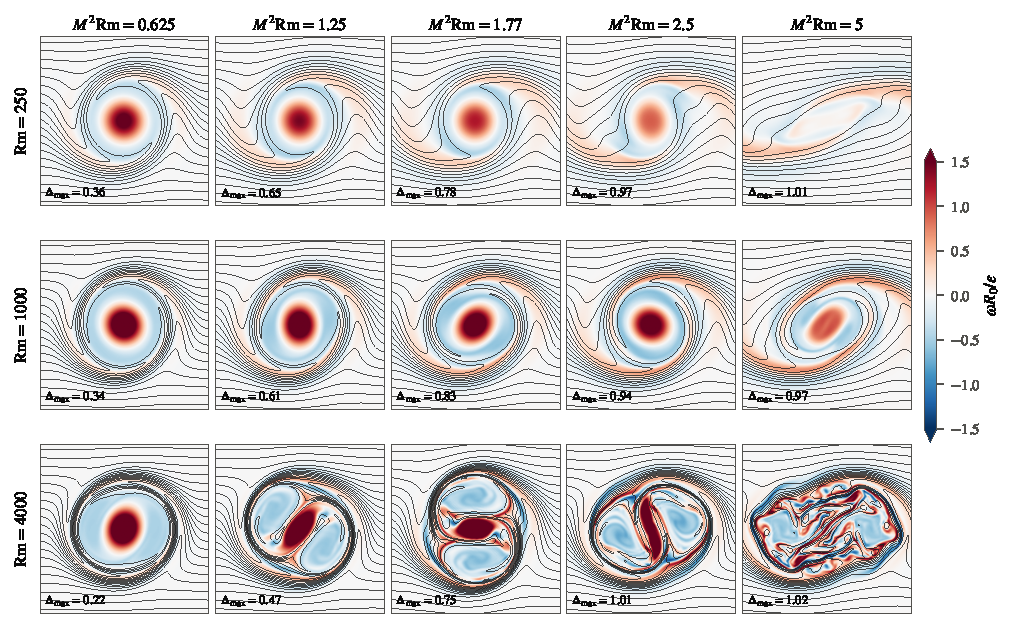
\includegraphics[width=\textwidth]{fig_gallery_t6}
\caption{The vortex at $t=6\Rm^{1/3}$ for $\Rm=\Rey=250$, $1000$, $4000$ (rows) and
$M^2\Rm=0.625$--$5$ (columns). Colour: vorticity; lines: magnetic field lines,
contours of the flux function every $0.5B_0R_0$. The central $10R_0$ of the
$20R_0$ box is shown. $R_0=20$ cells. $\Delta_\mathrm{max}$: the largest $\Delta$
in the run.}
\label{fig:g6}
\end{figure*}

\begin{figure*}
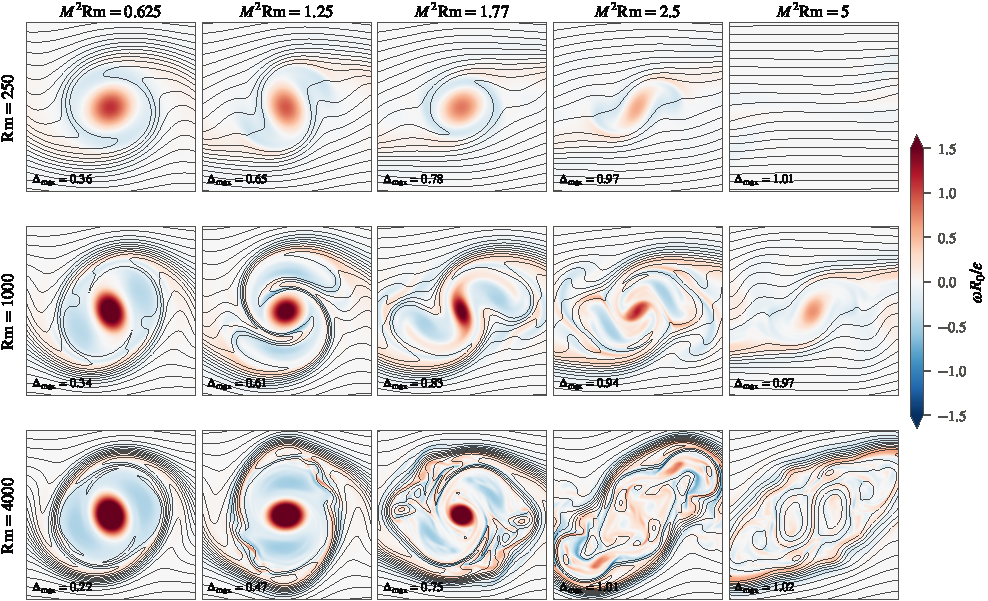
\includegraphics[width=\textwidth]{fig_gallery_t12}
\caption{As Fig.~\ref{fig:g6}, at the end of each run, $t=12\Rm^{1/3}$.}
\label{fig:g12}
\end{figure*}

\section{One field at three magnetic Reynolds numbers}

Figure~\ref{fig:fixed} follows the field $M^2\Rm=2.5$, above the threshold, at
$\Rm=\Rey=250$, $1000$ and $4000$, with time in units of $\Rm^{1/3}$. All three
vortices are destroyed, with largest $\Delta$ of $0.967$, $0.939$ and $1.005$. What
they lose during the wind-up is not the same: at $t=3\Rm^{1/3}$, $S=0.479$, $0.676$
and $0.796$. A fixed $M^2\Rm$ fixes the outcome and not the braking on the way to it,
which falls as $\Rm$ rises. At $\Rm=250$ the erosion of Sec.~I is visible; at
$\Rm=1000$ and $4000$ the tripole is.

\begin{figure*}
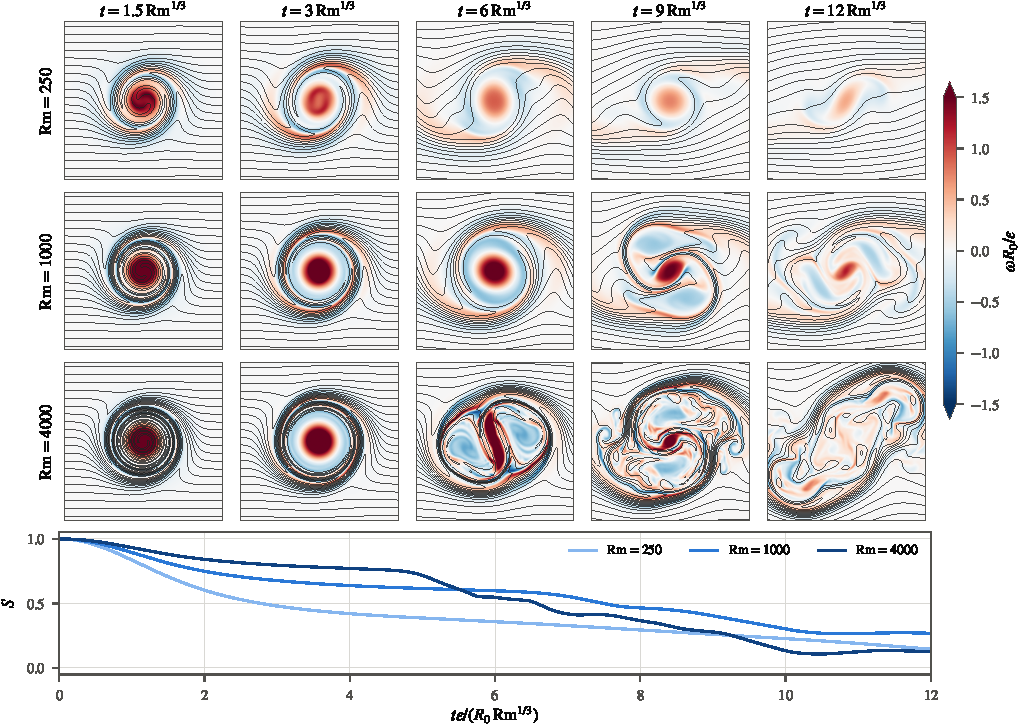
\includegraphics[width=\textwidth]{fig_fixed}
\caption{$M^2\Rm=2.5$ at $\Rm=\Rey=250$, $1000$ and $4000$ (rows) at
$t=1.5$, $3$, $6$, $9$ and $12\,\Rm^{1/3}$, and the survival $S$ of the three
against $t/\Rm^{1/3}$. $R_0=20$ cells.}
\label{fig:fixed}
\end{figure*}

\end{document}
